\chapter{Computational Study}
\label{ComputationalStudyChapter}

\epigraph{You don't really understand what you've got until you do a comprehensive model of it.}
{\textit{Christopher Tyler} \\ (Q\&A session at VSS 2019)}

\textit{The work presented here has been presented previously as a poster presentation at VSS 2018 \citep{garside_does_2018}\footnote{Poster available: \doi{10.6084/m9.figshare.6280865.v1}} and as an oral presentation at ICVS 2019 \footnote{Slides and abstract available: \doi{10.6084/m9.figshare.8832395.v1}}}.

\section{Summary}

% I am interested in the question of whether a melanopic signal might be useful for either estimating the illuminant(s) in a scene, or more directly transforming visual signals into an illuminant-independent space.

% Following initial psychophysical experiments, where results did not indicate a strong or simple relationship, I chose to take a step back and examine the problem that the HVS is faced with in a natural environment, which colour constancy solves. Through this route I hoped to answer the questions:
% \begin{enumerate}
% 	\item Would it be sensible for the HVS to use a melanopic signal to help solve this problem?
% 	\item If so, in what way would it be used?
% \end{enumerate}

Code is provided: \url{https://github.com/da5nsy/Melanopsin_Computational}

\section{Introduction}

In the other chapters of this thesis the approach taken to study the effect of melanopsin has mirrored standard practice: we think that melanopsin \emph{might} be involved in a specific process (for reasons that seem sensible enough) and so we run an experiment where we vary the amount of melanopsin activation within a stimuli and measure something to see if there is an associated change with the hope of understanding \emph{how} melanopsin might be involved, but at no point do we really drill down on the questions of \emph{why} melanopsin might be involved.

This has meant that it is unclear whether our results (positive or negative) can be taken at face value - perhaps our assumptions about what the benefits of a melanopsin-based signal were wrong, and we were consequently looking in the wrong place.

This chapter shall describe an exploratory computational study which took an ecological modelling approach to try and further our understanding of what, if any, benefits may arise by the use of a melanopsin-based signal for colour constancy.

\noindent The proposed benefits of this approach are: 
\begin{enumerate}
    \item It may be possible to answer the question of whether it is sensible in any way for melanopsin to be involved in colour constancy in any form whatsoever - is there any benefit to be had from involving melanopsin?
    \item We may be able to suggest or rule out specific computational structures - one computation might be beneficial whilst others might not be.
    \item It may be able to narrow the search area for future psychophysical experimentation - in previous experiments there have been lots of assumptions about the luminance range that melanopsin is active over, the spatial distribution (both in terms of receptive fields and influence over signals from distant parts of the retina), the temporal dynamics of the signals involved (and many other assumptions but conscious and unconscious). This is an opportunity to test whether a melanopsin-based signal is useful for specific ranges of the stimulus space over others, with the assumption that an interaction is more likely to exist in a manner which is advantageous to the host.
\end{enumerate}

\noindent The key research question for this section can be posed such:

\begin{quote}
Considering the conditions on our planet, \\
and the ecological requirements of vision, \\
would a signal from a melanopsin-expressing cell \\
be useful for colour constancy?
\end{quote}

This chapter shall give an overview of the main scripts which have been written, going through the logic and results of each. By doing this, a roughly chronological path of the thought processes involved will be presented.

%\section{melcomp\_1}

In melcomp\_1 three questions were initially proposed:
\begin{enumerate}
\item Considering only daylight spectra (excluding reflective surfaces for now), can a melanopic signal measure the chromaticity of daylight? % more precisely? as well as? in the same league?
\item Now considering also object reflectances, does a melanopic signal provide a means of calculating a sign and weight of shift required to counteract the chromatic shift induced upon objects by a change in daylight conditions?
\item Are there objects, or luminance levels, or daylight chromaticities for which the melanopic signal is particularly effective or ineffective at performing the above task?
\end{enumerate}

Foundational data consisting of 
the Granada daylight dataset 
\citep{hernandez-andres_color_2001}\footnote{Data: \url{http://colorimaginglab.ugr.es/pages/Data\#__doku_granada_daylight_spectral_database}},
the Stockman-Sharpe 10$^{\circ}$ cone fundamentals 
\citep{stockman_spectral_2000,stockman_spectral_1999}
(aka the CIE 2006 10$^{\circ}$ cone fundamental sensitivity functions \cite{cie_cie_2006})\footnote{Available as `T\_cones\_ss10' in \gls{PTB}.},
the melanopsin fundamental of \citet{lucas_measuring_2014}\footnote{Available as `T\_melanopsin' in \gls{PTB}.},
and a subset\footnote{For these computations 11 surfaces were chosen from the Vrhel dataset, with a roughly even representation of skin tones, fruit, and vegetable/greenery.} 
of the reflectances of \citet{vrhel_measurement_1994}\footnote{Available as `sur\_vrhel' in \gls{PTB}.}
were used.
% Many MANY other things were considered, but I think perhaps I'll summarise those elsewhere

Initial computations considered the illuminants alone, without considering the interaction with surface reflectances (as per question 1). However, to avoid repeating text and figures here both approaches (with and without reflectances) shall be considered alongside. Figures in this section use red to indicate `illuminant only' and grey for `illuminant with surfaces'. 

Tristimulus values $[L,M,S]$ and analogous melanopic values $I$ (as per standard tristumulus values but using the melanopsin fundamental) were computed as per eq X %
for each illuminant within the Granada dataset, and for each surface under each illuminant. A real-world version of the first set of values would be to measure a spectralon tile (or other uniformally reflective surface) under each daylight condition. \gls{MB} chromaticity co-ordinates were calculated, again for both illuminant alone and for each surface under each illuminant, as per equation X. %
The \gls{MB} chromaticities are plotted in Figure \ref{fig:MB}. Three-dimensional plots were made to display $l_{\text{MB}}$ against $s_{\text{MB}}$ against $[L,M,S,I]$ in turn. Each plot is shown in Figure \ref{fig:level1}. 

\begin{figure}[htbp]
    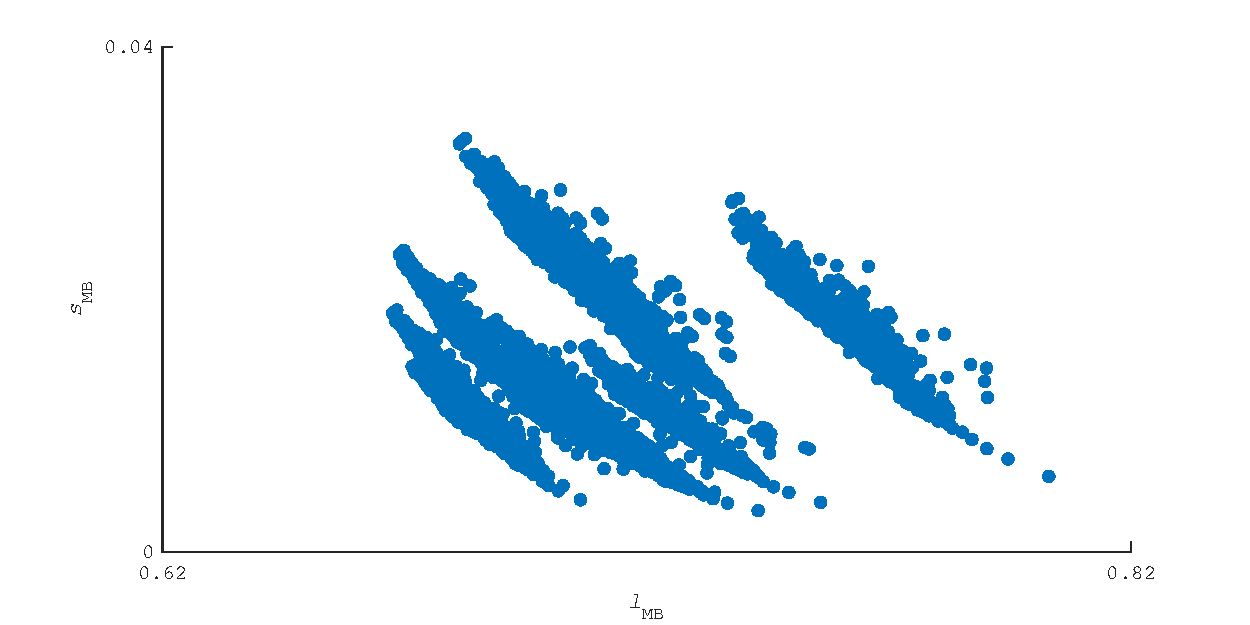
\includegraphics[max width=\textwidth]{figs/comp/melcomp_1/BasicMB.pdf}
    \caption{\gls{MB} chromaticities for 12 reflectances under 2600 daylight illuminants (grey-centred circles with colours denoting different surfaces, colours not linked to real colours, solely for visualisation), and chromaticities for illuminants alone (red-centred, black bordered circled).}
    \label{fig:MB}
\end{figure} 

\begin{figure}[htbp]
    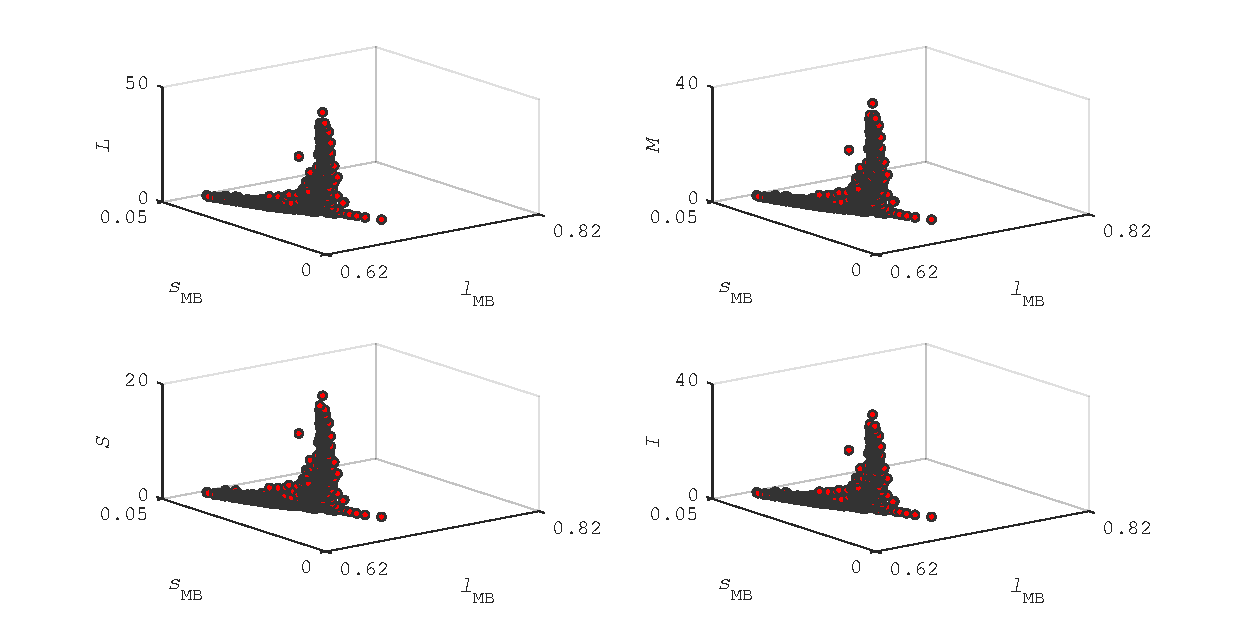
\includegraphics[max width=\textwidth]{figs/comp/melcomp_1/level1sigspredictingColorimetry.pdf}
    \caption{\gls{MB} chromaticity diagram on the horizontal plane ($l_{\text{MB}}$ against $s_{\text{MB}}$), with $[L,M,S,I]$ plotted in turn on the z-axis, for the illuminants of the Granada dataset, and a subset of the Vrhel reflectances. Red points indicate signals computed directly from the spectral power distribution, grey points represent values of computed colorimetry for objects under illuminants. Note - vertical axes rescaled per plot. For the red (illuminant only) points, in each graph the trend from left-to-right above is to start low with a gradual increase before fairly rapidly going vertical. Though hard to see here, the grey points follow the same trend, but on a surface-by-surface level.}
    \label{fig:level1}
\end{figure} 

From Figure \ref{fig:level1}, it can be seen that although there exists some relationship between the chromaticity values of the illuminants and the $[L,M,S,I]$ values, it does not appear as though one could be used to reliably predict the other. All that can be gained from this relationship is the understanding that if the $[L,M,S,I]$ value is above a certain threshold, it is likely to be in a group with a low $s_{\text{MB}}$ and high $l_{\text{MB}}$ value. The real-world correlate of this is - \textit{if the daylight is bright enough, I can be fairly confident that the chromaticity of light will be relatively warm in colour.} This is as expected, since the brightest daylight conditions are likely to be those with unobstructed direct sunlight, which is warmer in \gls{CCT} than illumination provided by the blue sky. This relationship seems relatively weak however, and could not be used to accurately predict the chromaticity of an illuminant. 

The answer to the first question set out for the script then, is that a melanopic signal cannot predict chromaticity (though neither can any other single signal). In regard to the second question, whilst a similar relationship is seen, it is on a surface-by-surface level (each group of points representing a single surface shows a similar trend to that highlighted in red for the illuminant-only points, but each group is distinct, though often overlapping, from others). The effect of this would be that for a random surface under a random illuminant, any of the $[L,M,S,I]$ values would do a poor job of predicting the chromaticity of the illuminant. The melanopsin-based value ($I$) certainly does not do a markedly better job than other values.

\begin{figure}[htbp]
    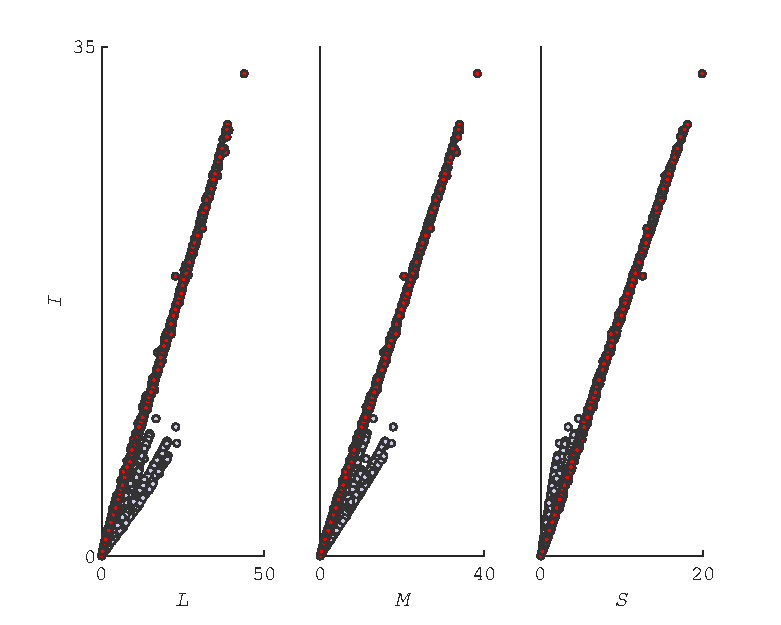
\includegraphics[max width=\textwidth]{figs/comp/melcomp_1/correlationBetweenLevel1Sigs.pdf}
    \caption{The relationship between melanopic power (analogous to a tristimulus value but calculated using the spectral sensitivity of melanopsin). Red points indicate signals computed directly from the spectral power distribution, grey points represent values of computed colorimetry for objects under illuminants.  The traditional tristimulus values show a very strong correlation for illuminant-only values. It is not particularly easy to see here, but each surface is represented by a roughly straight line of grey points at slightly different angles.}
    \label{fig:tristimCorrelation}
\end{figure} 

It should be noted that there was very high correlation between each signal. This is shown in Figure \ref{fig:tristimCorrelation} and the correlation table below. This can be considered as corresponding to the high importance of the first principal component of the spectral measurements in this dataset. Put another way, a sensor with almost any spectral sensitivity could be used to estimate the general magnitude of the daylight. The discussion of principal components shall be returned to under melcomp\_3.

%\begin{minipage}{\linewidth}
\begin{lstlisting}
corr(LMSI)
    1.0000    1.0000    0.9993    0.9998
    1.0000    1.0000    0.9995    0.9999
    0.9993    0.9995    1.0000    0.9999
    0.9998    0.9999    0.9999    1.0000
\end{lstlisting}
%\end{minipage}

\bigskip

Following this, similar plots were made which plotted $l_{\text{MB}}$ against $s_{\text{MB}}$ as before, but now plotted the various combinations of $[L,M,S,I]$, created by considering one signal over another (e.g. $L/M$), on the z-axis. These plots are shown in Figure \ref{fig:allComboSignals}. Following the terminology of \citet{barrionuevo_contributions_2014} $[L,M,S,I]$ shall be referred to as `first level signals' and these derived signals as `second level signals'. The twelve plots created all showed clear and relatively simple relationships between chromaticity and these new derived signals, at least for the illuminant-only values. Again, a similar trend was seen for each individual surface, but once surfaces were included any overall trend broke down into small replicants of the overall trend.
% This might end up putting a single line on a page. Check before submitting

% \clearpage
% 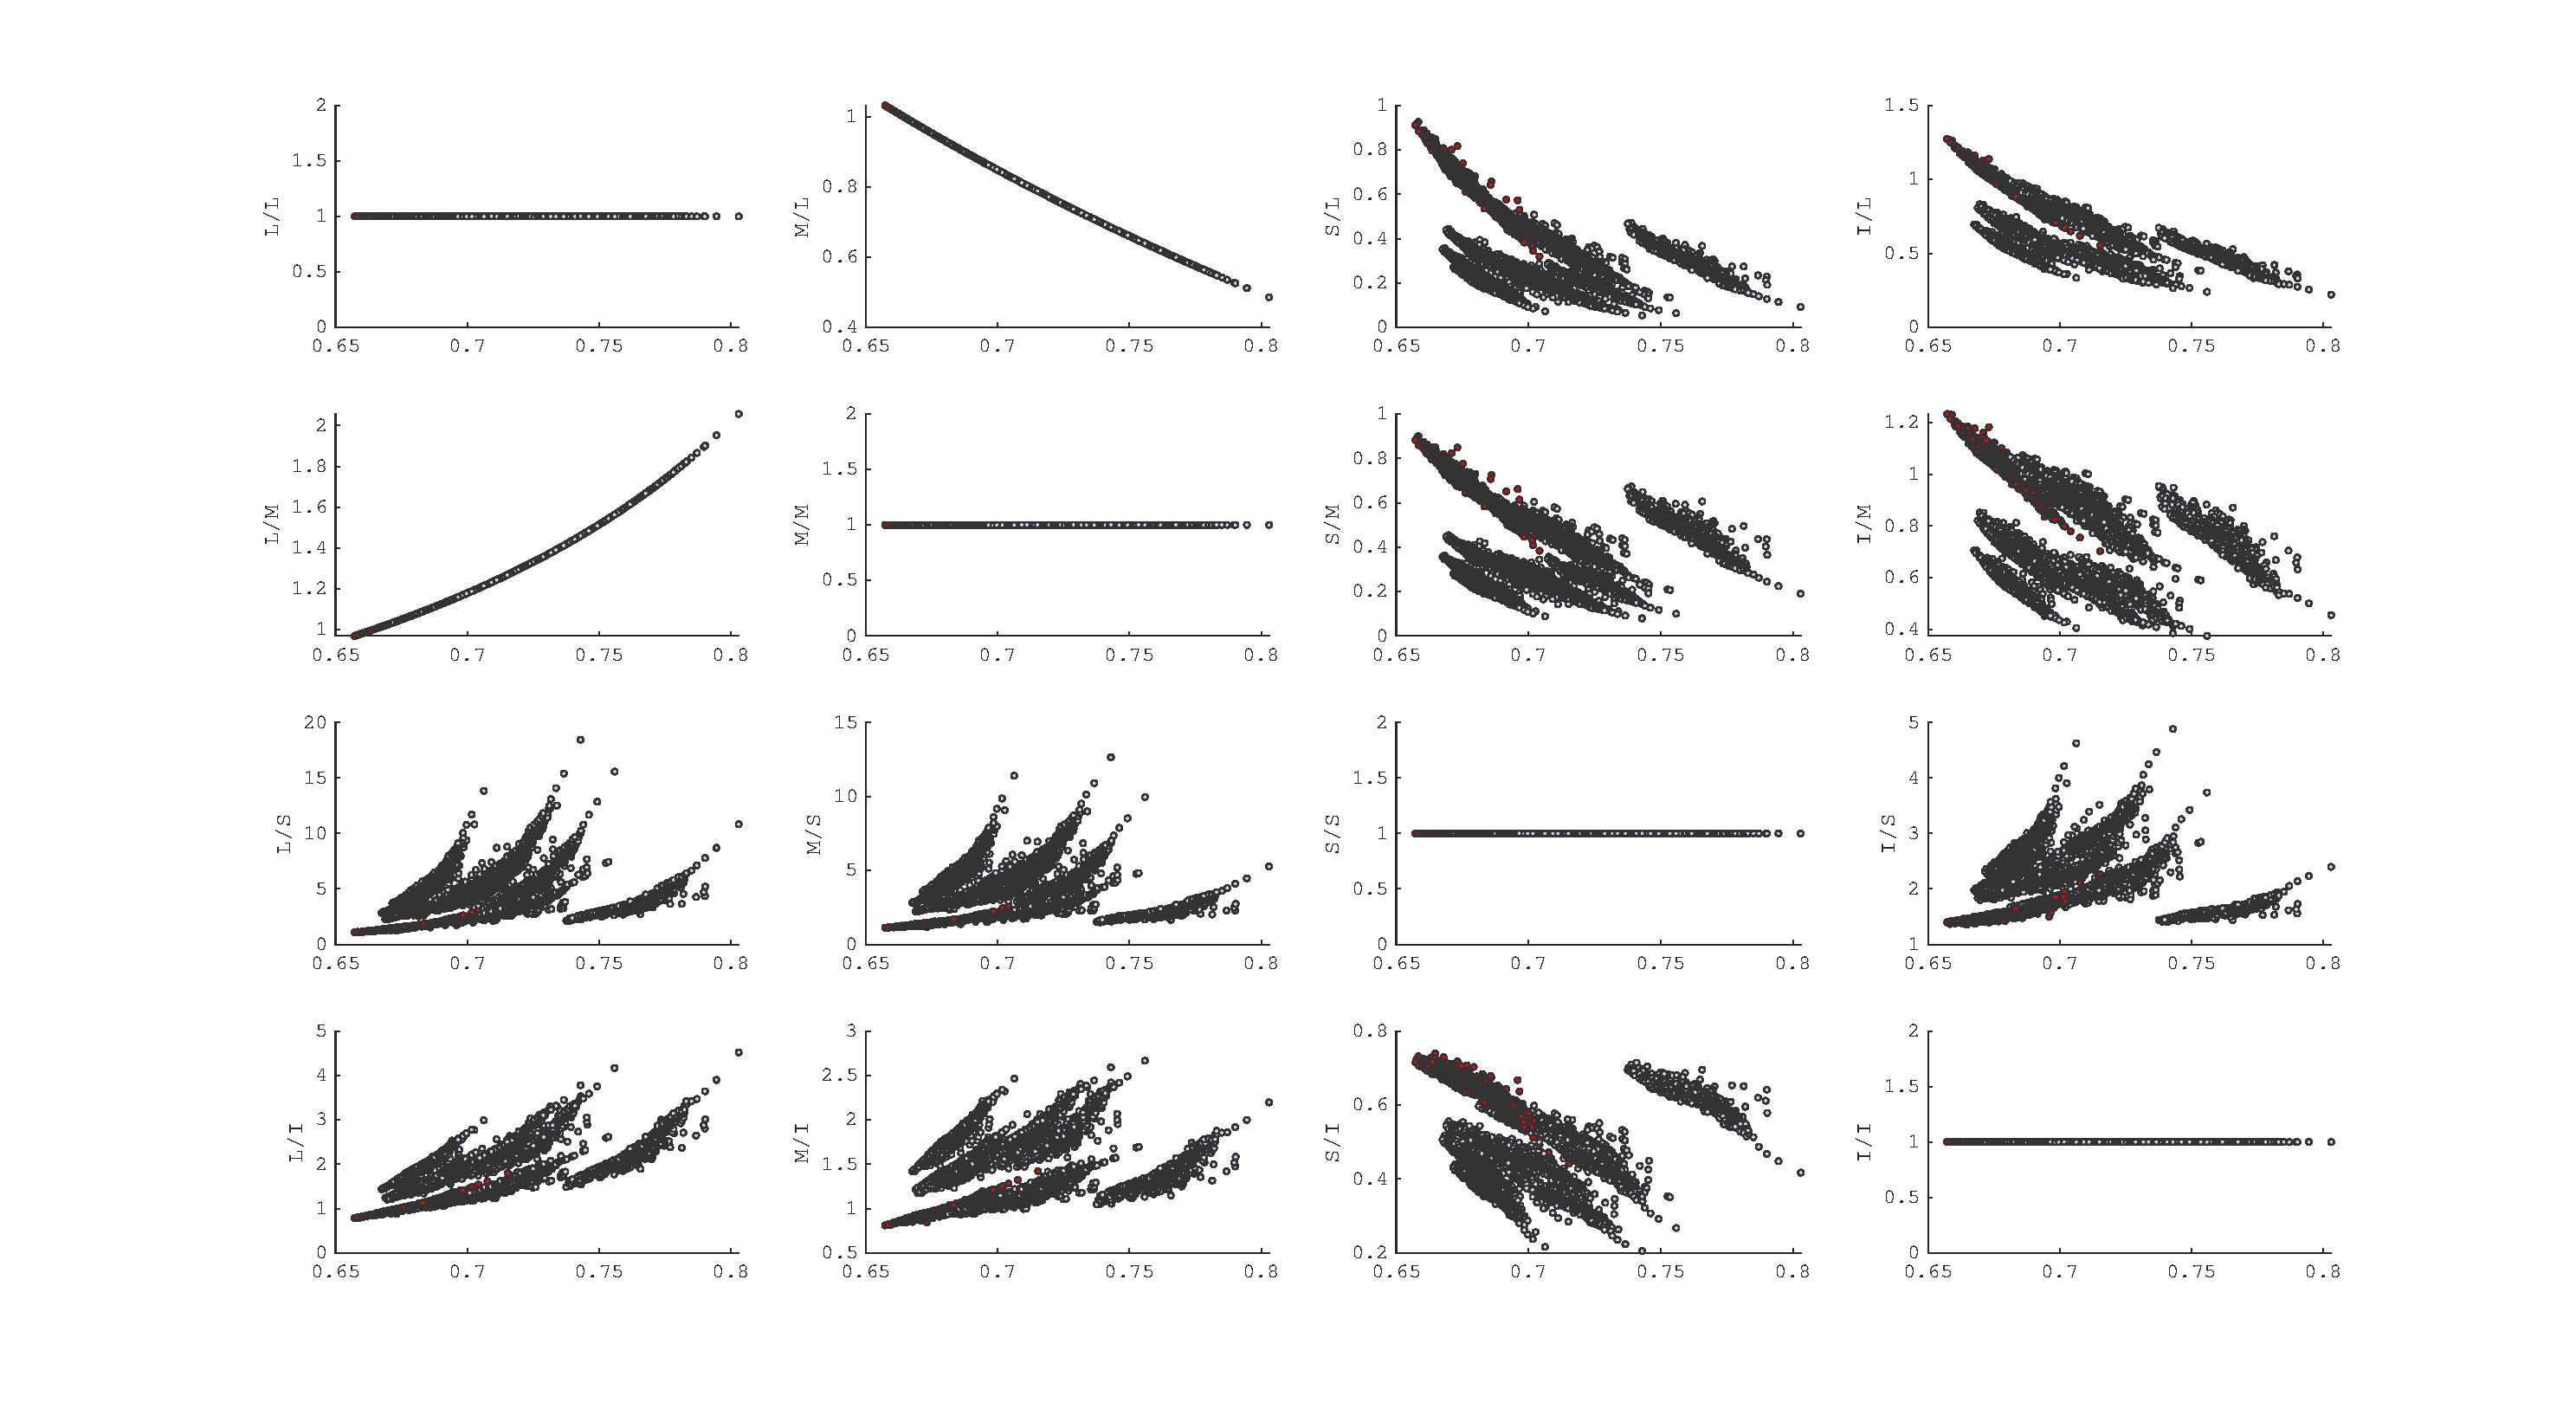
\includepdf[pages=-,rotate=90, offset=75 -75]{figs/comp/melcomp_1/allComboSignals.pdf}
% \begin{figure}[h!]
%     \caption{Relationship between chromaticity and second level signals. Plotted on the x-axis here is $l_{\text{MB}}$, with second level signals on the apparent y-axis. During analysis these plots were three dimensional, with the apparent y-axis being a z-axis and the x-axis joined by a y-axis of $s_{\text{MB}}$. As before, red points indicate signals computed directly from the spectral power distribution, grey points represent values of computed colorimetry for objects under illuminants. It can be seen that on a per object basis (incl. no object) there is good correlation between all of the above signals (though often it is non-linear).}
%     % See gifs online at...
%     \label{fig:allComboSignals}
% \end{figure} 
% %\clearpage
% % does it look weird if this doesn't spread over a double?


\begin{fullpagefigure}
\figpdf[pages=-,rotate=90, offset=75 -75]{figs/comp/melcomp_1/allComboSignals.pdf}
\caption{Relationship between chromaticity and second level signals. Plotted on the x-axis here is $l_{\text{MB}}$, with second level signals on the apparent y-axis. During analysis these plots were three dimensional, with the apparent y-axis being a z-axis and the x-axis joined by a y-axis of $s_{\text{MB}}$. As before, red points indicate signals computed directly from the spectral power distribution, grey points represent values of computed colorimetry for objects under illuminants. It can be seen that on a per object basis (incl. no object) there is good correlation between all of the above signals (though often it is non-linear).}
% See gifs online at...
\label{fig:allComboSignals}
\end{fullpagefigure}

For many of these signals however, such relationships are to be expected\footnote{My thanks go to Manuel Spitschan for convincing me of this point.}. For example, a relationship between $l_{\text{MB}}$ and $L/M$ should be expected, since $l_{\text{MB}}$ is defined as the sum of weighted components of $L$ and $M$. To confirm this, a null condition was performed, where $[L,M,S,I]$ was replaced by randomly generated values, and the second level signals were generated as before. The results can be seen in Figure \ref{fig:allComboSignals_rand}. Relationships between secondary signals derived from $L$, $M$ or $S$ signals still showed correlations with chromaticity (albeit now points fell on a plane, instead of a line), whereas signals with a $I$ component showed only minimal coherence, forming a noisy cloud in three-dimensional space. This implies that should the melanopic signals correlate with chromaticity, that this is not simply a computational artefact of the way in which chromaticity is calculated.

% \clearpage
% 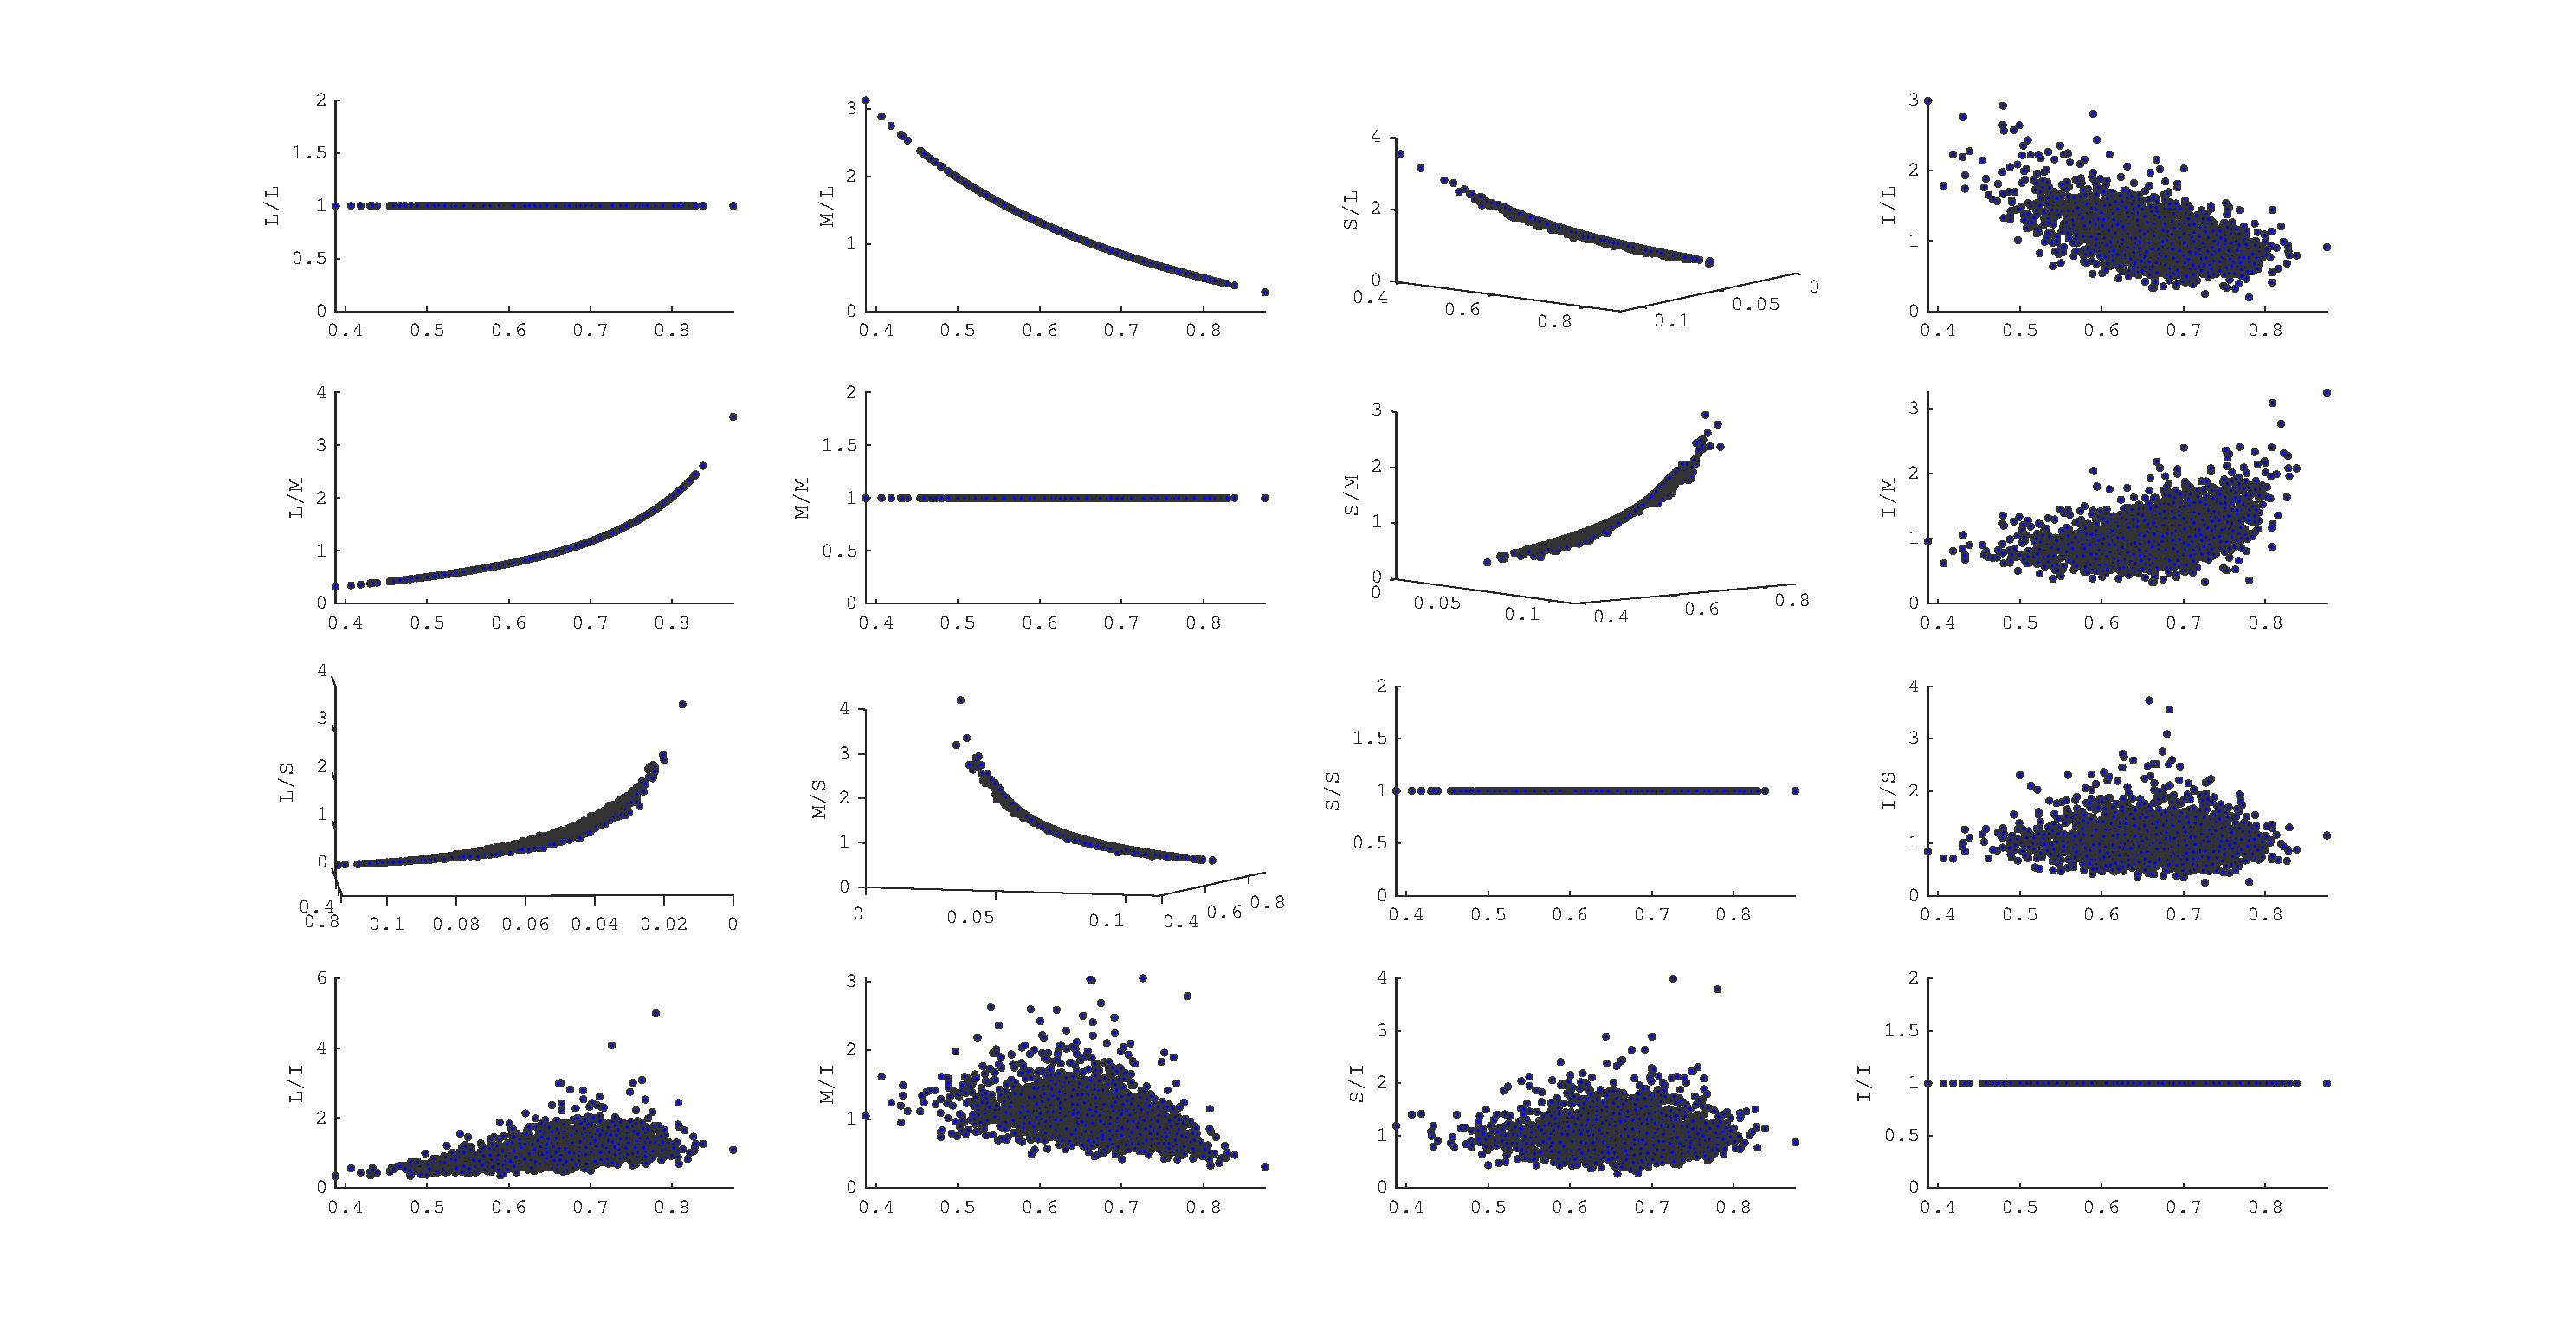
\includepdf[pages=-,rotate=90, offset=75 -75]{figs/comp/melcomp_1/allComboSignals_rand.pdf}
% \begin{figure}[h!]
%     \caption{As per \ref{fig:allComboSignals} but where $[L,M,S,I]$ was replaced by randomly generated values, and the second level signals were generated from these instead of real values. Where relationships still exist, this implies that they are computational artefacts rather than underlying relationships. Blue is used to distinguish this random data from previous real data. Note that different rotations have been applied to some of the subplots to best display the correlations.}
%     \label{fig:allComboSignals_rand}
% \end{figure} 
% %\clearpage
% % does it look weird if this doesn't spread over a double?



\begin{fullpagefigure}
\figpdf[pages=-,rotate=90, offset=75 -75]{figs/comp/melcomp_1/allComboSignals_rand.pdf}
\caption{As per \ref{fig:allComboSignals} but where $[L,M,S,I]$ was replaced by randomly generated values, and the second level signals were generated from these instead of real values. Where relationships still exist, this implies that they are computational artefacts rather than underlying relationships. Blue is used to distinguish this random data from previous real data. Note that different rotations have been applied to some of the subplots to best display the correlations.}
\label{fig:allComboSignals_rand}
\end{fullpagefigure}

This example shows that if a melanopic signal exhibits correlation with a chromatic signal \emph{not} due to the underlying mathematics of how chromaticity is calculated, and that any relationship must follow from a genuine regularity in the data.

Considering question 2 more closely, rather than just looking for a correlation with chromaticity, it was considered whether it was possible to perform a conversion of the computed surface chromaticities into an abstract illuminant-independent space, using a melanopic value as a corrective signal. Considering that the absolute melanopic values seemed to offer little predictive benefit (see Figure \ref{fig:level1}) the choice was made to create a normalised melanopic value similar in nature to the MB values. Following equation X % 
but with a melanopic value in place of the $S$ value allowed for the creation of what shall be termed the $i_{\text{MB}}$ values.

It was found through an optimisation procedure that through addition and subtraction of weighted $i_{\text{MB}}$ values, using the scaling factors shown in equation \ref{eq:correction} such a conversion could approximately be performed. The optimisation sought optimal weights for the scaling factors with the goal of minimising the overall spread of chromaticities (measured as standard deviation of the entire set\footnote{Spoiler: this was a bad idea.}). The effect of different weights can be seen in Figure \ref{fig:minSD}. The results of applying equation \ref{eq:correction} can be seen in figure \ref{fig:corrected}.

\begin{subequations} \label{eq:correction}
\begin{align}
l_{\text{MB}}* &= l_{\text{MB}} + 0.30i_{\text{MB}}\\ %these will have changed
s_{\text{MB}}* &= s_{\text{MB}} - 0.21i_{\text{MB}}
\end{align}
\end{subequations}

\begin{figure}[htbp]
    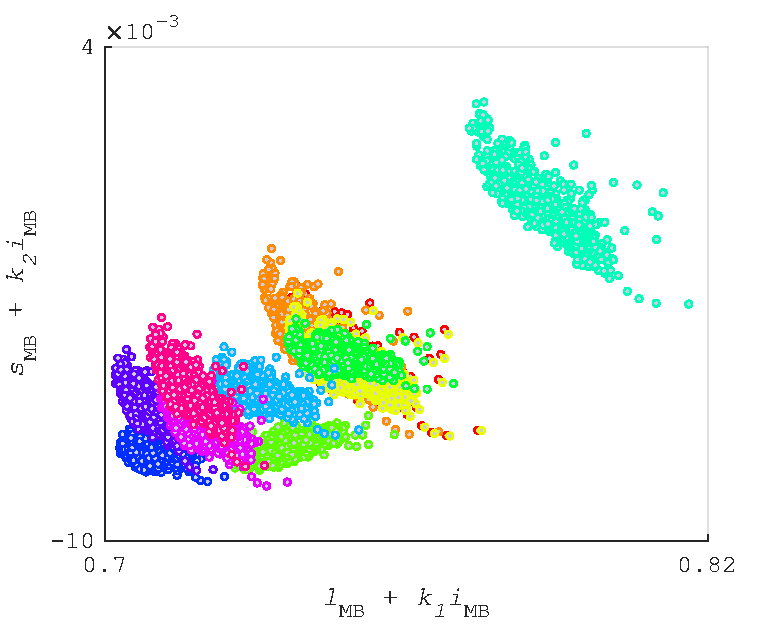
\includegraphics[max width=\textwidth]{figs/comp/melcomp_1/correctedChromaticities.pdf}
    \caption{\gls{MB} chromaticities for 12 reflectances under 2600 daylight illuminants, corrected by the corresponding $i_{\text{MB}}$ value.}
    \label{fig:corrected}
\end{figure} 

It can be seen that the points now roughly cluster together by object, with less smearing induced by changes in illuminant (compared to Figure \ref{fig:MB}).

It was unclear however, whether any additional signal would provide such an advantage. With this in mind, a further optimisation procedure was performed, to consider whether shifting the sensitivity of the melanopsin function along the wavelength spectrum affected the performance of such a signal. Each new sensitivity function was allowed the benefit of the first type of optimisation, allowing different scaling factor weights. The results of this optimisation can be seen in figure \ref{fig:opt}. It can be seen that minima for $l_{\text{MB}}$* occur at around 530nm and just under 600nm, and minima for $s_{\text{MB}}$* occur at around 450nm and 580nm. On first appearance this seems to suggest that the optimal spectral sensitivity for a cone type employed to correct the signals from the various cones might be around these points in the spectrum. However, the reader might note the correspondence between the figures above and the peak spectral sensitivities of the cones themselves (S-448nm, M-541nm, L-569nm). Indeed we see that the optimal performance occurs when the nominal melanopsin sensitivity overlaps most well with the spectral sensitivity of the cones. It is understandable why this occurs - each signal is then normalised by a near-duplicate of itself, rendering each value in the set being close to zero. Since we set the goal of the optimisation procedure to be the reduction of the standard deviation of the \emph{entire set}, the optimisation finds these near-duplicate values to be very effective.

\begin{figure}[htbp]
    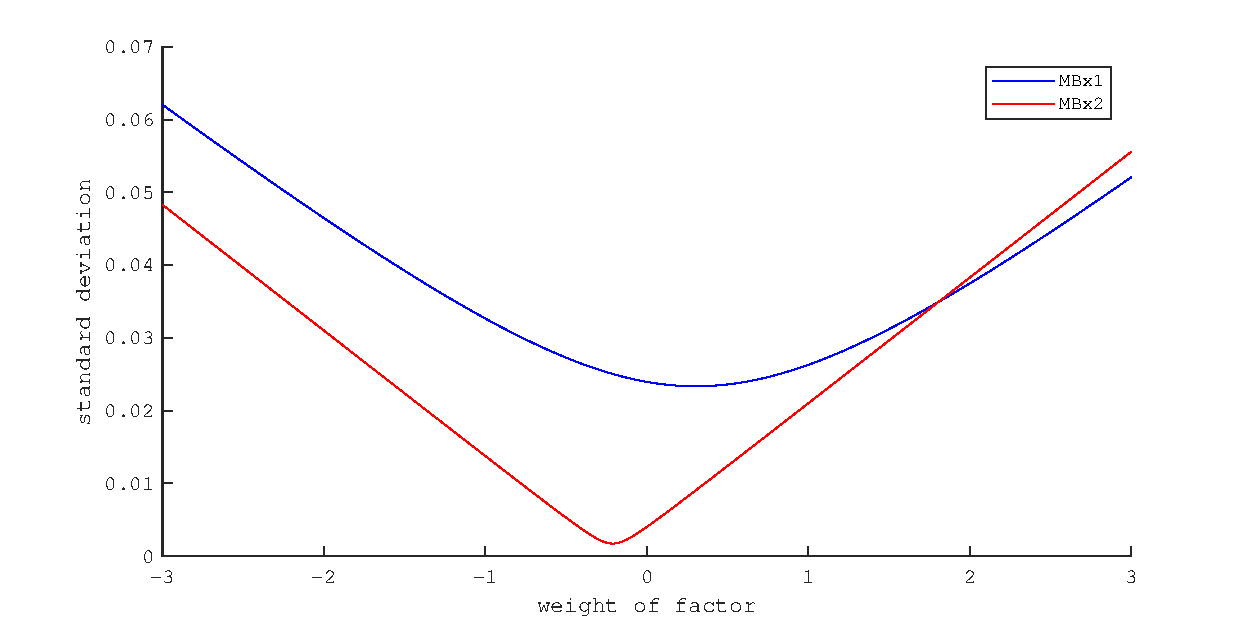
\includegraphics[max width=\textwidth]{figs/comp/melcomp_1/minimiseSD.pdf}
    \caption{A plot showing the optimal minima for the factor weights.}
    \label{fig:minSD}
\end{figure} 

\begin{figure}[ht]
    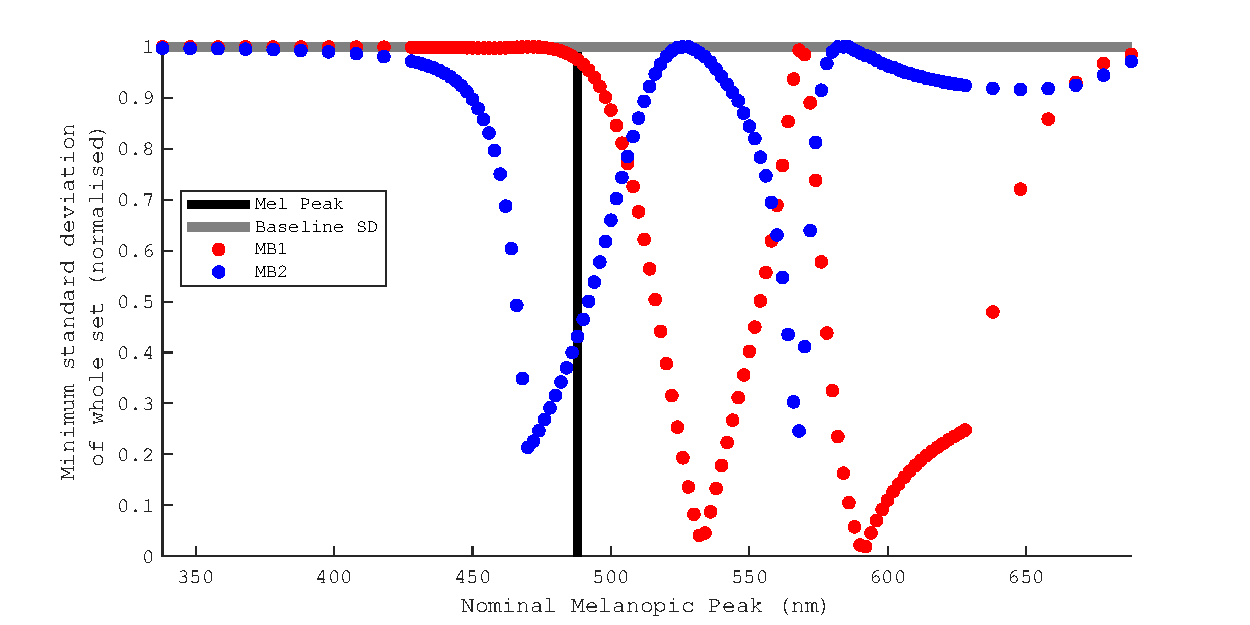
\includegraphics[max width=\textwidth]{figs/comp/melcomp_1_caller/opt.pdf}
    \caption{The results of an optimization where the spectral sensitivity of the nominal melanopsin fundamental was shifted along the spectrum. Generated using melcomp\_1\_caller.m for iteration.}
    \label{fig:opt}
\end{figure} 

Using these values had the unexpected and unfortunate effect of simply crushing all the chromaticties down onto a single line, without preserving any inter-object chromatic differences. We witness perfect colour constancy, at the expense of any chromatic discrimination\footnote{At my poster at VSS David Brainard referred to this as the 'Ford Model of Colour Constancy' - you can have any colour, so long as it's black}. This is obviously not ideal.

\begin{figure}[htbp]
    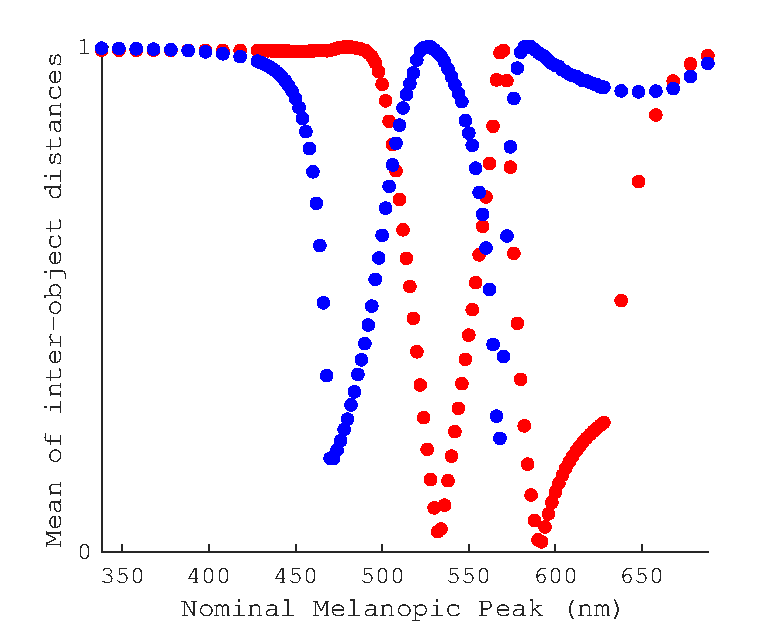
\includegraphics[max width=\textwidth]{figs/comp/melcomp_1_caller/sdmeans.pdf}
    \caption{Normalised average distance between points in the set of the mean chromaticities for the different reflectances. It can be seen that inter-reflectance variation drops to zero at the same minima as seen in figure \ref{fig:opt}, showing that these distinct points are undesirably corrected to the same point. Generated using melcomp\_1\_caller.m for iteration.}
    \label{fig:sdmeans}
\end{figure} 

\textit{The work was presented at this stage as a poster at the \emph{Vision Science Society Conference (VSS)} in 2018.}

The actual desired behaviour would be to minimise internal variance for each reflectance group, whilst maintaining at least some distinction between inter-reflectance groups. A comprehensive approach to this question would need to consider the relative importance of the two separate requirements, and apply appropriate weightings. This idea is returned to in melcomp\_X. %!!!!!!!!

To summarise melcomp\_1, and address the questions laid out at the start:
\begin{enumerate}
    \item A basic melanopic signal, computed from direct daylight measurements, cannot predict chromaticity, other than a crude estimation of whether a measurement is direct sunlight or not. \emph{Figure \ref{fig:level1}}
    \item The same can be said for melanopic values computed for daylight reflected off a surface. \emph{Figure \ref{fig:level1}}
    \item A first level melanopic value is highly correlated with first level cone signals. \emph{Figure \ref{fig:tristimCorrelation}}
    \item There are relatively strong relationships between hypothetical second level signals (\emph{Figure \ref{fig:allComboSignals}}) but some of these appear to be nothing more than computational artefacts (\emph{Figure \ref{fig:allComboSignals_rand}}). Notably, the melanopic second level signals did not suffer in this way.
    \item A basic corrective procedure was applied, which seemed to reduce the spread of chromaticities. \emph{Figure \ref{fig:corrected}} 
    \item It was found that when the melanopic value was replaced by signals generated from different spectral sensitivities, and passed through the same optimisation procedure, the best performing signals were near-duplicates of existing signals. These signals performed very well judged by our metric of entire set standard deviation, but in practice would make very poor corrective signals. \emph{Figure \ref{fig:sdmeans}}
    \item The stage at which consideration of which objects/luminance levels/daylight chromaticities a melanopic signal might be best/worst suited for was not reached. Further development required.
\end{enumerate}

\section{melcomp\_2}

Following VSS I changed my perspective on the problem slightly and started to think more deeply about the $i_{\text{MB}}$ signal as a third dimension upon the already two-dimensional \gls{MB} chromaticity space, such as shown in figure \ref{fig:ZL}. This allowed me to consider what properties a signal upon this third dimension would need to provide to the overall three-dimensional point cloud in order for a transformation to occur which would transform the values into a two-dimensional illuminant-independent space.

\begin{figure}[htbp]
 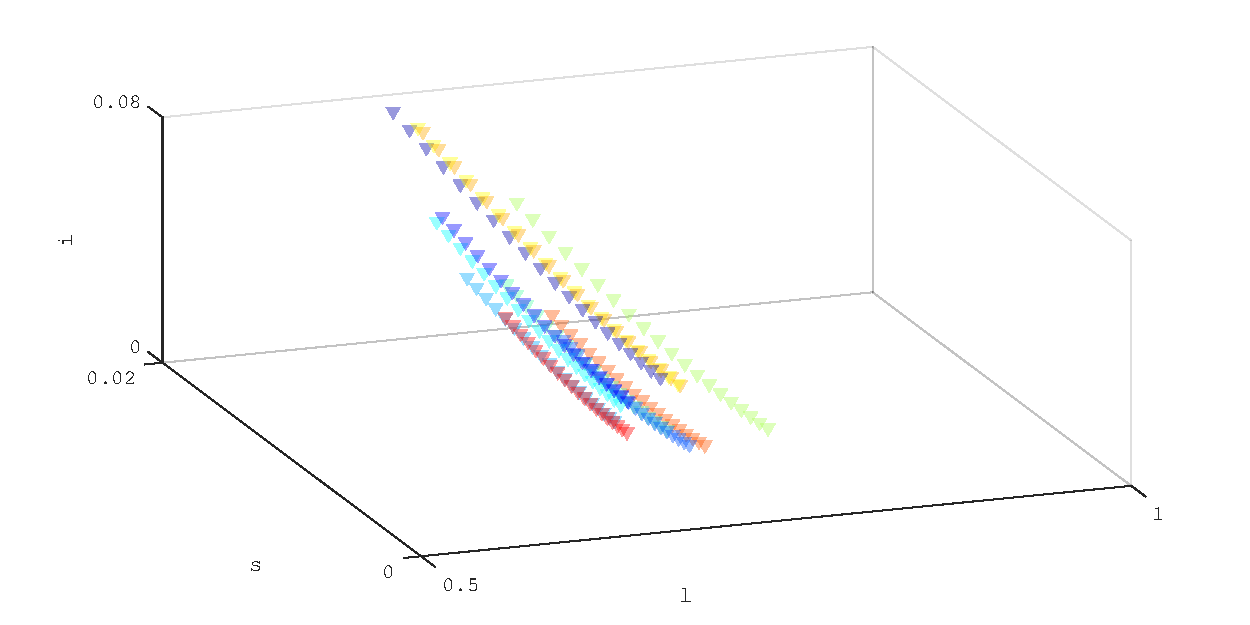
\includegraphics[max width=\textwidth]{figs/comp/melcomp_2/ZL.pdf}
 \caption{X and Y axes are a \gls{MB} chromaticity space, derived in this case using the \gls{SP} fundamentals, and the Z axis is $i_{\text{MB}}$. Plotted are the values for 11 surfaces (as per melcomp\_1), under 20 D-series illuminants (non-linear range between 3600 and 25000).}
 \label{fig:ZL}
\end{figure} % Update axes to add `MB'

The script started with the same process as melcomp\_1, loading data and computing \gls{MB} chromaticities, along with hypothetical $i_{\text{MB}}$ values. $r_{\text{MB}}$ values, the rod based analogue, were also calculated, although this was done for completeness (again, following the influence of \cite{barrionuevo_contributions_2014}) rather than following a genuine belief that they could be involved.

In addition to the data considered in melcomp\_1, support was added to consider a range of CIE D series illuminants\footnote{Generated with the \gls{PTB} function `GenerateCIEDay'.}, the scenes 1-4 of the
\citet{nascimento_statistics_2002}\footnote{Data: \url{https://personalpages.manchester.ac.uk/staff/d.h.foster/Hyperspectral_images_of_natural_scenes_02.html}} hyperspectral reflectance data,
scenes 1-5 of the 
\citet{foster_frequency_2006}\footnote{Data: \url{https://personalpages.manchester.ac.uk/staff/d.h.foster/Hyperspectral_images_of_natural_scenes_04.html}}
hyperspectral reflectance data, and the \gls{SP} fundamentals\footnote{Loaded through \gls{PTB} as `T\_cones\_sp' (the new version as of \url{https://github.com/Psychtoolbox-3/Psychtoolbox-3/commit/2d360a2e827ed03174206cada5717ee555c727a1}).}. The CIE D-series illuminants allowed for a smaller and more controlled dataset, the Foster et al. data allowed for a more realistic distribution of reflectances and the \gls{SP} fundamentals allowed for a technically `correct' \gls{MB} diagram (before I knew about CIE 170-2:2015 \cite{cie_cie_2015}).

\hl{There's a log transform here that I haven't mentioned yet\dots}

The key finding at this stage was that there is a perspective upon a three-dimensional point cloud ($[l_{\text{MB}},s_{\text{MB}},i_{\text{MB}}]$) from which points from like objects clustered well, such as in figure \ref{fig:viewpoint}. This property shows that there is at least one transformation such that the points could be projected upon a two-dimensional plane where the illuminant dependence was greatly reduced whilst the inter-object chromatic relationships were retained. 

\begin{figure}[htbp]
 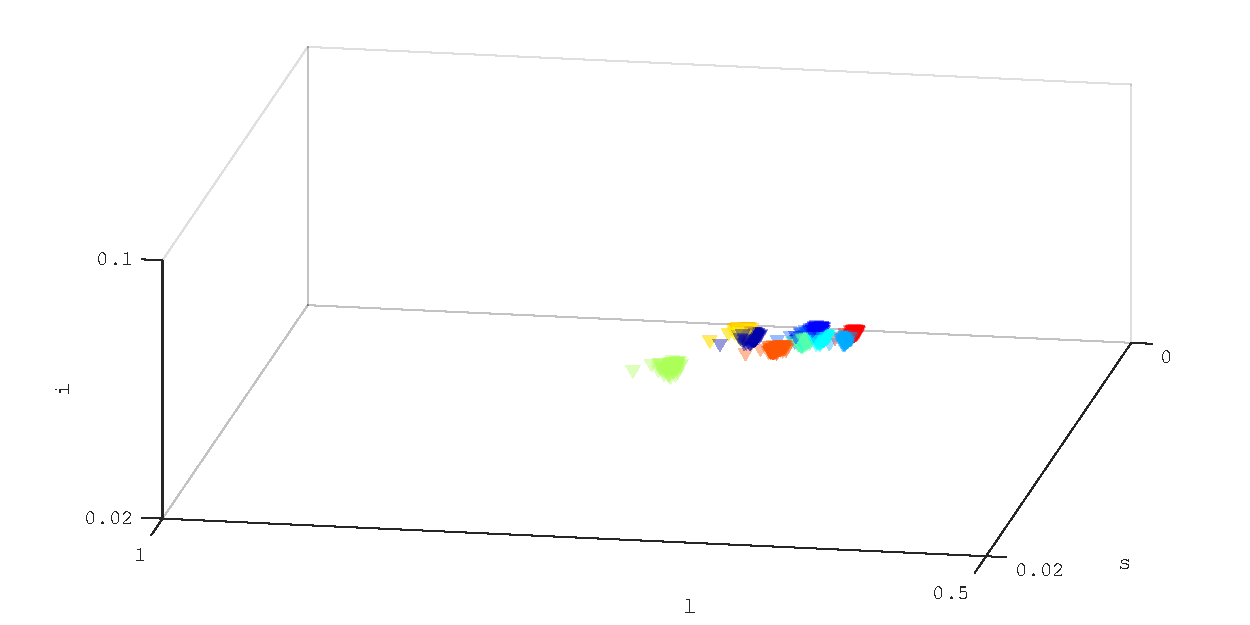
\includegraphics[max width=\textwidth]{figs/comp/melcomp_2_caller/viewpoint.pdf}
 \caption{Figure \ref{fig:ZL} rotated to a perspective where it can be seen that the points project upon a two-dimensional plane in a clustered fashion whilst not degrading to a line within that space.}
 \label{fig:viewpoint}
\end{figure} 

Note that such a perspective would not be possible for a space where the third dimension were a duplicate of the first or second, since in this case all points would lie upon a plane. This would be the case in circumstances where a corrective signal too closely resembled the visual signals, as we found at the end of melcomp\_1. The fact that points do not lie on a plane shows that there is some decorrelation between $i_{\text{MB}}$ and both $l_{\text{MB}}$ and $s_{\text{MB}}$. The fact that they do not lie on a plane and instead diverge from this plane in a surface-dependent fashion (as opposed to noisily diverging) suggests that the $i_{\text{MB}}$ may present a means to seperate the contribution from illuminant and surface, which is really exciting.

Following this, a range of speculative transformations were performed, to demonstrate the types of transformation that could be used to transform colour signals to illuminant-independent colour signals. A rotational transformation was successful (analogous to changing the perspective as in figure \ref{fig:viewpoint}) and additionally a weighted additive model was found to be more-or-less successful. No satisfactory model was found where a purely multiplicative transformation was applied.

Thinking about a corrective signal as an additional dimension upon a \gls{MB} chromaticity space allows for consideration of requisite or desirable properties that this third signal should imbue upon the three-dimensional cloud of points. I have identified one requisite property, and one desirable property. 

The requisite property for such a signal, as already suggested, is that it should differ from other chromatic signals enough to allow for the point cloud of chromatic points to be significantly \emph{non-planar}. This in turn allows for a projection upon two-dimensional space which has the potential to be illuminant-invariant.

The desirable property is that it should be \emph{roughly monotonic} with respect to other chromatic signals. This allows a one-to-one mapping of colour signals to illuminant-independent colour signals, where a non-monotonic relationship does not necessarily do so. This is not a strict requirement, since the corrective function only needs to be one directional, but non-monotonicity would exclude simple transforms (such as linear additive or rotational).

At this stage I thought thinking about the underlying reason for the relative success of these transforms. One potential lead is a curious regularity at the lower wavelengths of the reflectance spectrum of many natural objects. In figure \ref{fig:plateau} it can be seen that there is a plateau in the relative spectral reflectances of some natural objects (a subset of the \citet{vrhel_measurement_1994} reflectances) between roughly 430nm and 480nm, with relatively small deviations within 400nm to 500nm. Another way to visualise this is to calculate the correlation between points on the reflectance function. Such a calculation was performed initially on a combined set of scenes 1-4 of the
\citet{nascimento_statistics_2002}\footnote{Data: \url{https://personalpages.manchester.ac.uk/staff/d.h.foster/Hyperspectral_images_of_natural_scenes_02.html}} hyperspectral reflectance data and
scenes 1-5 of the 
\citet{foster_frequency_2006}\footnote{Data: \url{https://personalpages.manchester.ac.uk/staff/d.h.foster/Hyperspectral_images_of_natural_scenes_04.html}}
hyperspectral reflectance data, and then on three other datasets. See figure \ref{fig:foster} and \ref{fig:others} respectively.

\begin{figure}[htbp]
 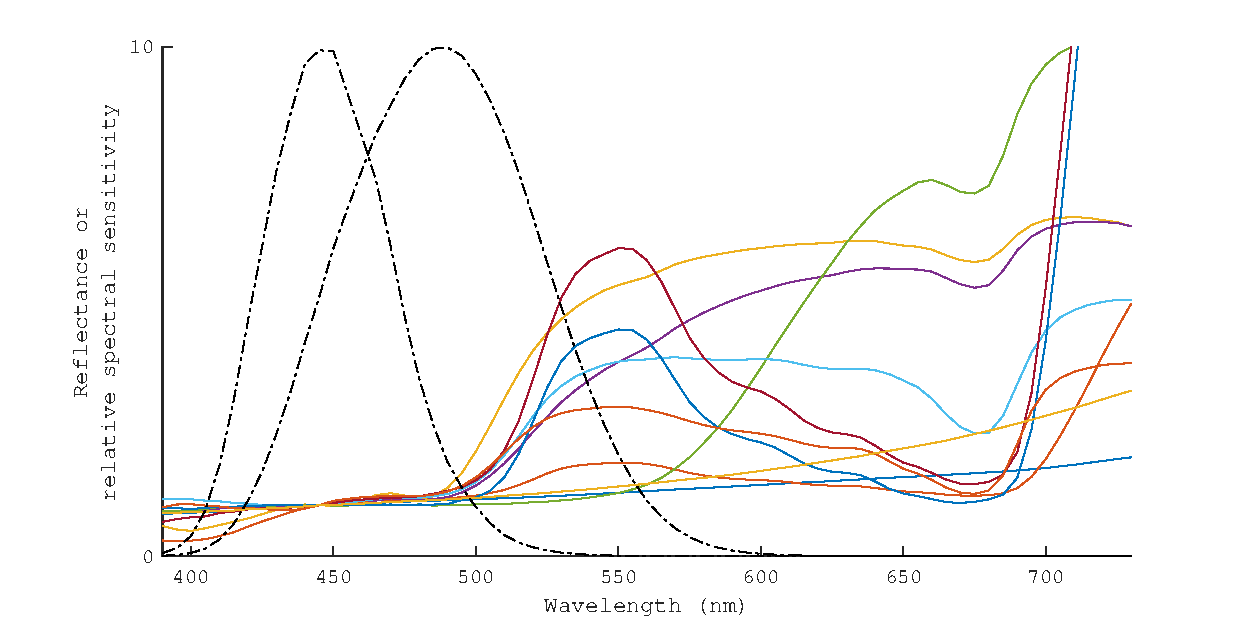
\includegraphics[max width=\textwidth]{figs/comp/melcomp_2_caller/plateau.pdf}
 \caption{The spectral reflectance functions of a subset of the \citet{vrhel_measurement_1994} reflectances (solid lines), normalised at the peak of s-cone sensitivity (CIE 2006 10$^{\circ}$), with the spectral sensitivity of s-cones and melanopsin \citep{lucas_measuring_2014} overlaid (dot-dashed lines).}
 \label{fig:plateau}
\end{figure} 

\begin{figure}[htbp]
 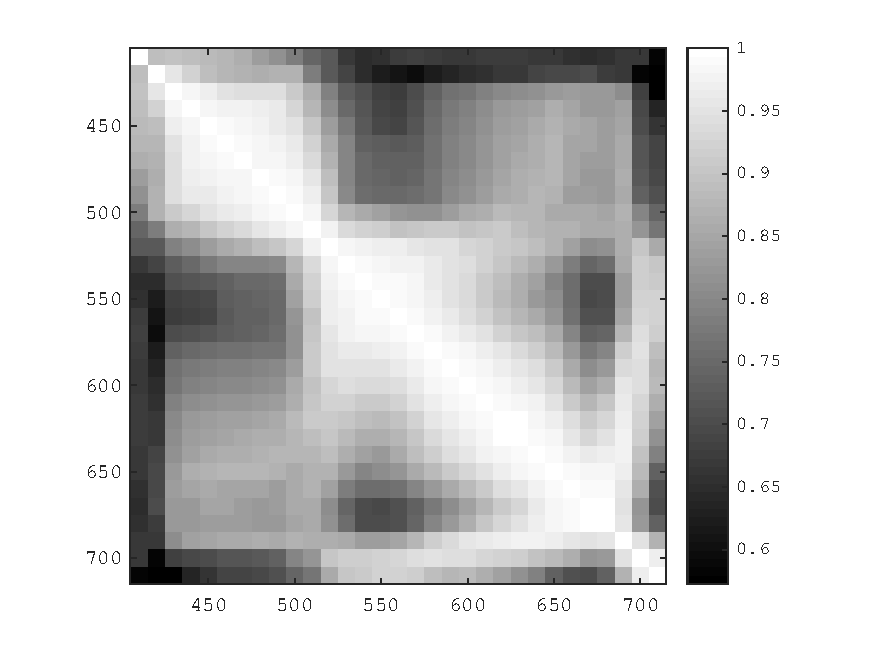
\includegraphics[max width=\textwidth]{figs/comp/nat_cor/foster.pdf}
 \caption{Visualisation of the average correlation matrix for the scenes 1-4 of \citep{nascimento_statistics_2002} and 1-5 of \citep{foster_frequency_2006}. Note the rough square in the top left, indicating an area of increased correlation across different wavelength samplings, and another rough square (though with a faded lower-right corner) in the centre. The dark frame to this figure is likely due to increased measurement noise at these extremes.}
 \label{fig:foster}
\end{figure} %get rid of dotted line on colorbar

\begin{figure}[htbp]
 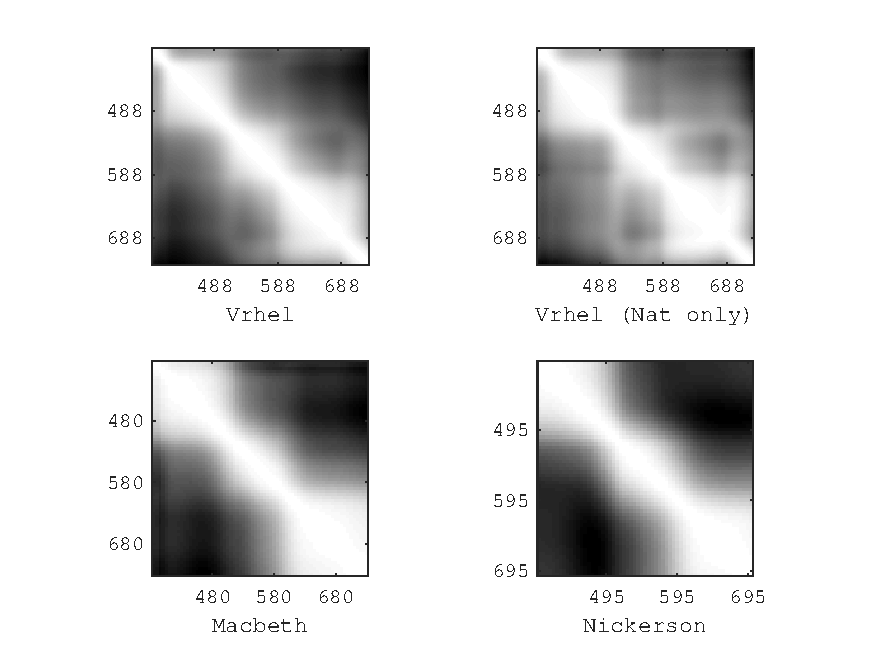
\includegraphics[max width=\textwidth]{figs/comp/nat_cor/others.pdf}
 \caption{As for \ref{fig:foster} but for 3 different sets of data, and one subset. `Vrhel' refers to the object reflectances of \citet{vrhel_measurement_1994} data and `Vrhel (nat only)' refers to a subset of the previous but only using data for surfaces which were deemed `natural'. `Macbeth' refers to measurements of a Macbeth Color Checker. `Nickerson' refers to a set of measurements of Munsell papers (presumably the \citet{kelly_tristimulus_1943} data). Note that whilst we have a selection of real surfaces, natural surfaces, and printed papers, all plots show similar trends, with three areas of correlation, at low, medium and high wavelengths. The low wavelength square seems to match that in Figure \ref{fig:foster} well, but the other two areas are only really distinguishable in this second set of figures. All data obtained via \gls{PTB} (`sur\_vrhel', `sur\_macbeth', `sur\_nickerson').}
 \label{fig:others}
\end{figure} 

An interesting advantage could be made of this regularity. Assume a simpler situation where there were two points on the spectrum of the reflectance functions of a set of natural objects which were always the same as eachother (perfect correlation). Sensors of appropriately narrow spectral sensitivity, placed at these two points on the spectrum would always register corresponding signals. Considering that the second principal component of daylight variability is a broad skew, any difference in the signals from two such receptors could be used fairly reliably to sense the contribution of this second component in any single condition. 

This work was presented at this stage as a poster at the \emph{Visual Neuroscience Summer School (Rauischholzhausen, 2018)} as a poster, which has not been made publicly available.

\section{melcomp\_3}

At the Visual Neuroscience Summer School I spoke with Laurence Maloney about this work, and about his own work on colour constancy \citep{maloney_computational_1984,maloney_color_1986}, and he suggested that I consider a simple game: given cone catches from an unknown surface under an unknown illuminant, guess the illuminant. If you are able to guess the illuminant with a moderate accuracy, you've cracked colour constancy.

Whilst this had been an implicit thread throughout much of the work to this point, it was a neat idea to be spelled out so clearly. I had my reservations - from my experience with the rotational corrective transform (Figure \ref{fig:viewpoint}) I had seen that a correction (to an illuminant-independent space) seemed possible even without explicit knowledge of the illuminant. Of course one could get an estimate of the illuminant from such a computation, but it was a potential output, not a requisite input. All the same, I thought it would be a relatively neat and simple thing to show.

In melcomp\_3 I attempt this, using the framework of linear modelling which Laurence is so well known for. It is used in a relatively rudimentary way here, compared to the complex manner in which Laurence uses it in his thesis \citep{maloney_computational_1984}. Whereas there he uses it to compute a solution to colour constancy, here I only use it to define my light sources, and then query which signals can predict the light sources so defined.

I start in much the same way as I have done in melcomp\_1 and 2, by loading data upon which to perform the computations. This time, I used an extended subset of the \citet{vrhel_measurement_1994} dataset, considering anything which could be considered natural rather than the small selection previously needed, on the basis that to consider correlation I would need an increased number of datapoints. At this stage I was using the \gls{SP} fundamentals, mainly in order to obey the rules of the traditional \gls{MB} diagram \citep{macleod_chromaticity_1979}. Again I used the Granada data \citep{hernandez-andres_color_2001}. From these inputs, I compute the $[L,M,S,R,I]$ values, and the corresponding \gls{MB} chromaticity values and pseudo-MB values ($i_{\text{MB}}$ and $r_{\text{MB}}$) for each surface under each illuminant.

I also compute the principal component representation of each illuminant. A variable weighting was specified, which gave most importance to wavelengths between the peak sensitivity of the S-cones and the peak sensitivity of the L-cones, before tailing off at each end (shown in Figure \ref{fig:VW}). This weighting is an important and difficult choice, and no entirely sensible solution is forthcoming\footnote{Do we care more about certain wavelengths than others? Yes. Which ones and by how much by? Unknown, and evolutionarily circular.}. \citet{maloney_evaluation_1986} discusses this further. %read and say more

% \begin{figure}[htbp]
%  \includegraphics[max width=\textwidth]{figs/comp/melcomp_3/?.png}
%  \caption{The variable weightings applied during the \gls{PCA} analysis. Generated by tracing the upward ramp of the S-cone sensitivity being used, plateauing at unity until the decrease of the L-cone sensitivity, and then following the decrease of the L-cone sensitivity.}
%  \label{fig:VW}
% \end{figure} 

The principal components identified are shown in Figure \ref{fig:PCA}. The first three components account for X,Y, and Z\% of variance respectively.

% \begin{figure}[htbp]
%  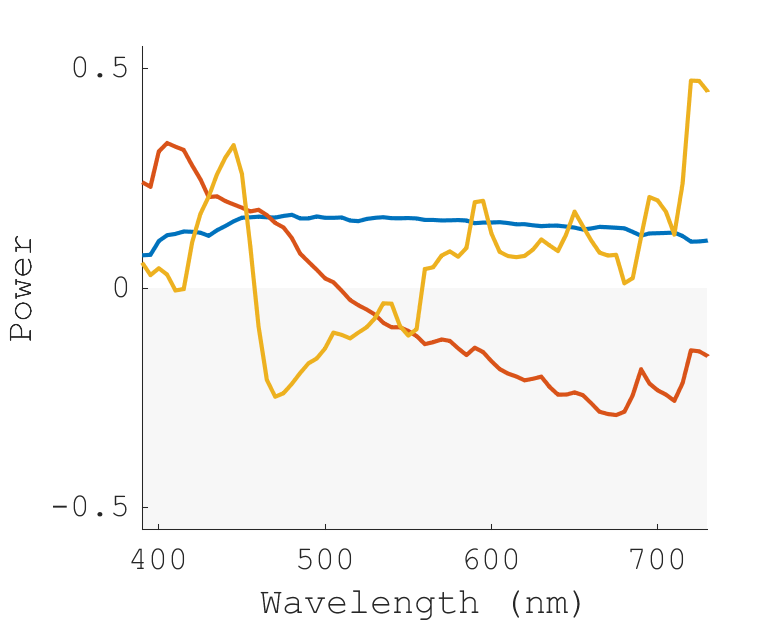
\includegraphics[max width=\textwidth]{figs/comp/melcomp_3/8.png}
%  \caption{The first 3 principal components for the Granada daylight dataset, conditional on the variable weighting shown in Figure \ref{fig:PCA}.}
%  \label{fig:VW}
% \end{figure} 

% Might be neat to show the chromatic effect of each of these PCs?

I then computed the correlation between a large number of candidate signals and the scores for different components of the \glspl{SPD}. This is shown in \ref{fig:19}. Plain talk: which signal was best at predicting each element of the daylight spectra upon a scene?

% \begin{figure}[htbp]
%  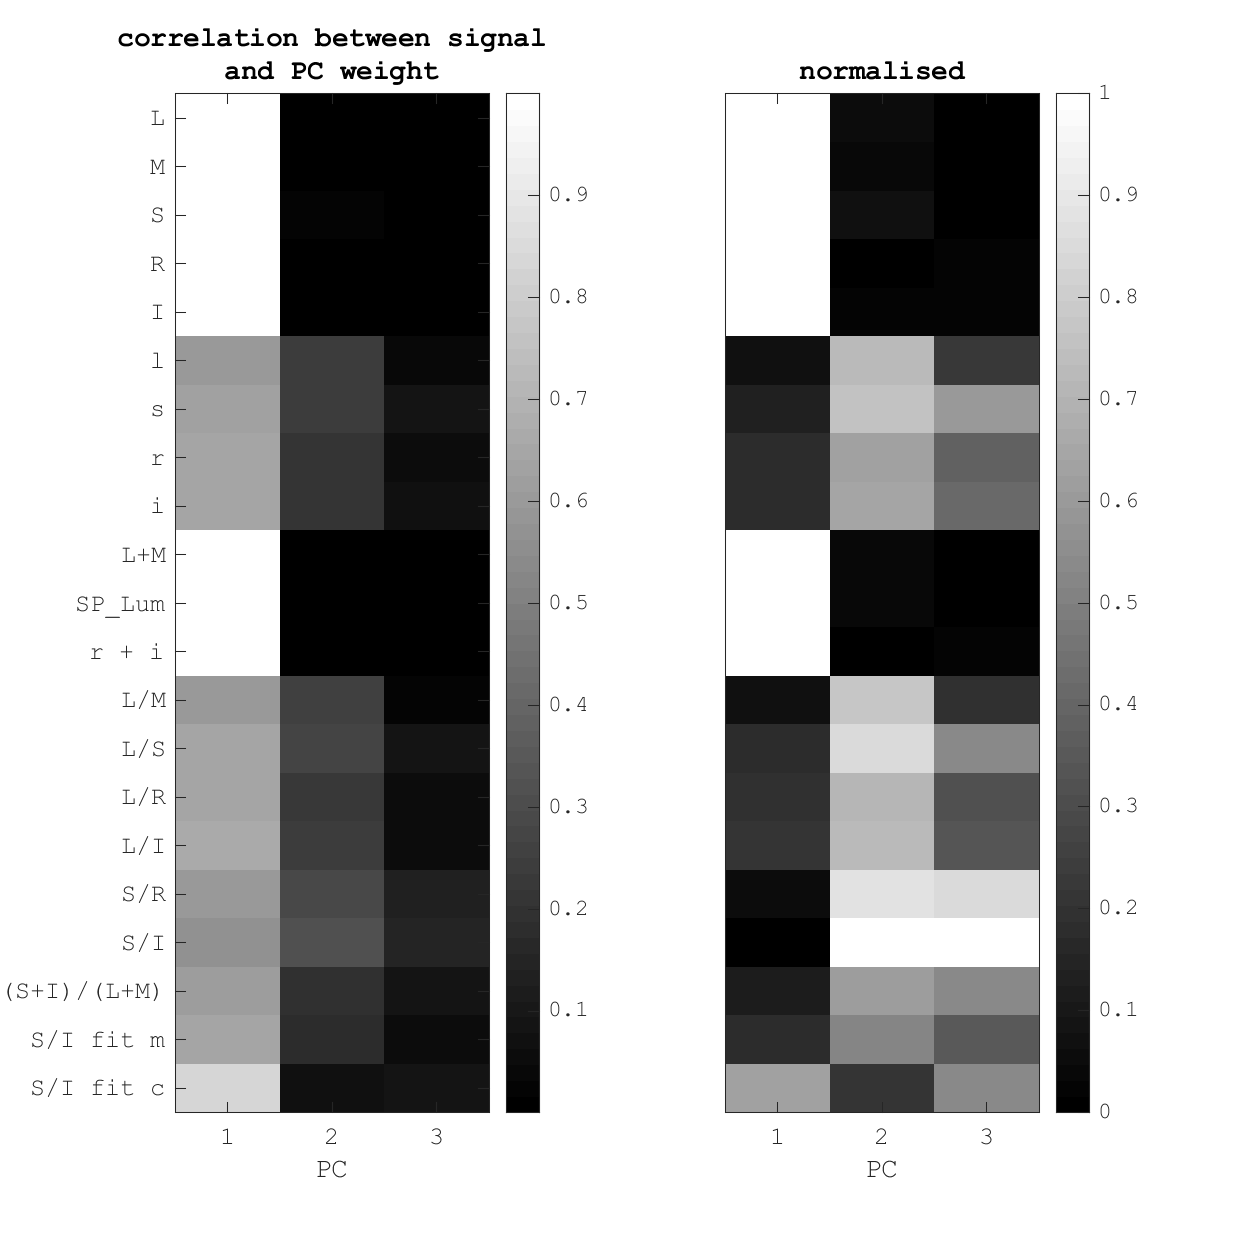
\includegraphics[max width=\textwidth]{figs/comp/melcomp_3/19.png}
%  \caption{\hl{Caption}}
%  \label{fig:19}
% \end{figure} 

% \begin{figure}[htbp]
%  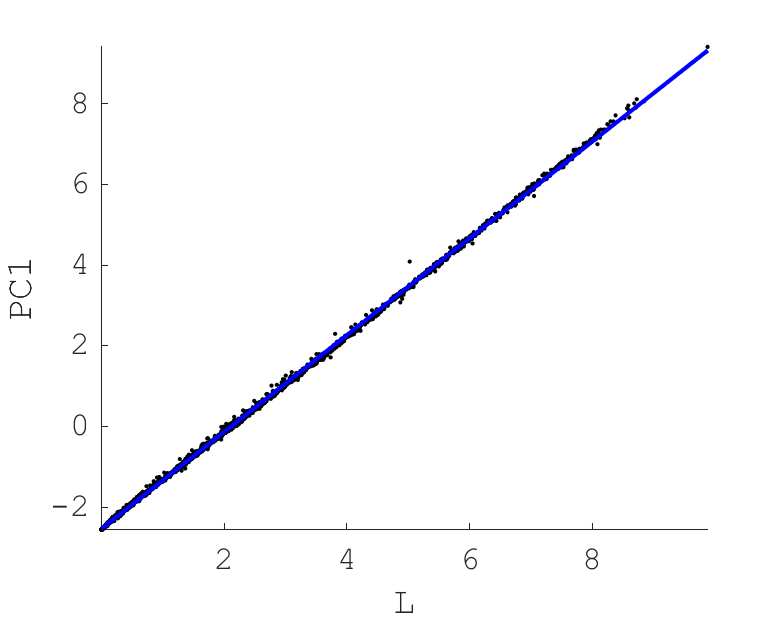
\includegraphics[max width=\textwidth]{figs/comp/melcomp_3/20.png}
%  \caption{\hl{Caption}}
%  \label{fig:L-PC1}
% \end{figure} 

% \begin{figure}[htbp]
%  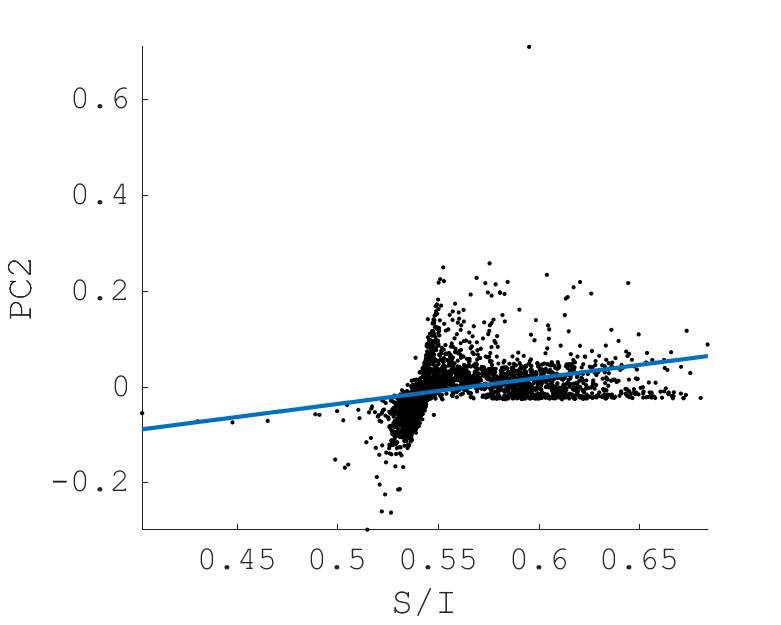
\includegraphics[max width=\textwidth]{figs/comp/melcomp_3/21.png}
%  \caption{\hl{Caption}}
%  \label{fig:S/I-PC2}
% \end{figure} 







% In melcomp\_3 I dove I approached the problem with a linear models approach, drawing on the work of Maloney \hl{refs!}. This is so far a bit of a bust, but I'm hoping that as I bring it all together it might click into place.


%\begin{figure}
%     \centering
%     \begin{subfigure}[b]{0.49\textwidth}
%         \centering
%         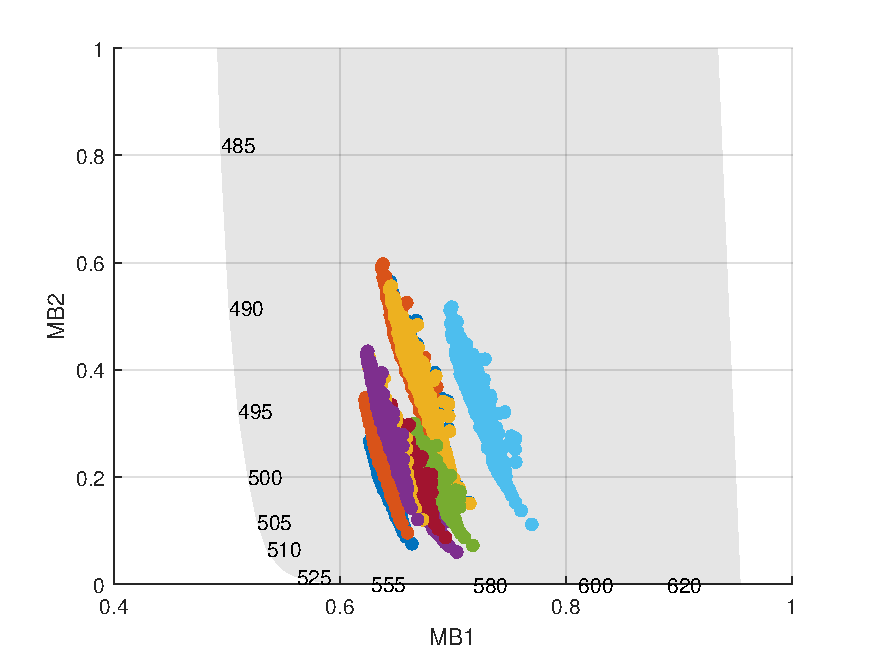
\includegraphics[width=\textwidth]{figs/mb.pdf}
%         \caption{$y=x$}
%         \label{fig:y equals x}
%     \end{subfigure}
%     \hfill
%     \begin{subfigure}[b]{0.49\textwidth}
%         \centering
%         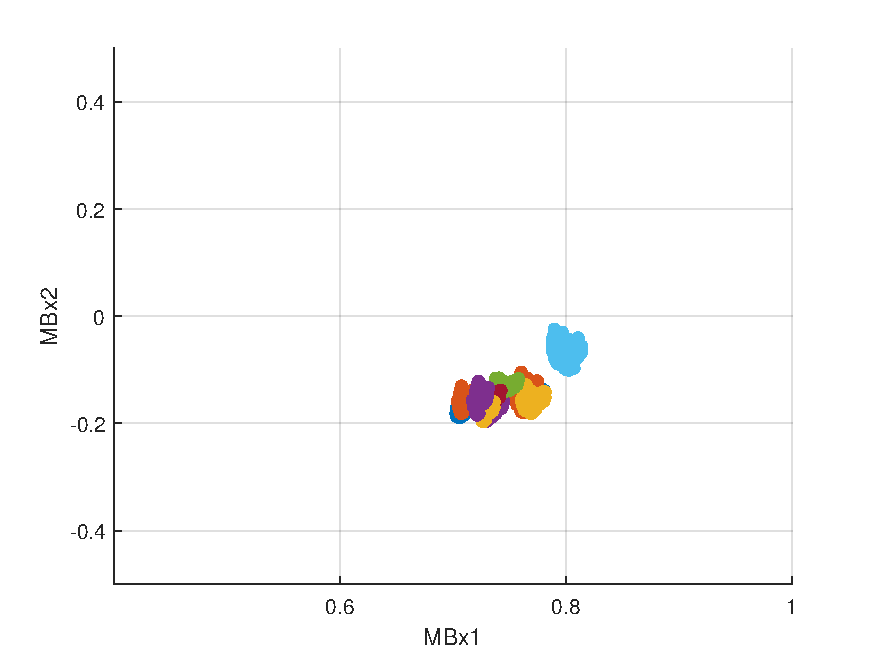
\includegraphics[width=\textwidth]{figs/corrected.pdf}
%         \caption{$y=3sinx$}
%         \label{fig:three sin x}
%     \end{subfigure}
%     \hfill
%        \caption{Three simple graphs}
%        \label{fig:three graphs}
%\end{figure}

